% Summary index document for the analysis chapter
\chapter{Analyse}
\label{chap:Analyse}

In diesem Kapitel wird unsere Wahl der Pcap-Bibliothek erläutert.
In diesem Kapitel wird unsere Wahl der Programmiersprache und \acs{PCAP}-Library erläutert.

<<<<<<< HEAD
\section{Vergleich von Java und Go}
\label{sec:Vergleich von Java und Go}

\subsection{Performancetest}
Die beiden Sprachen wurden mithilfe einer Testumgebung verglichen um Performanceunterschiede festzustellen. Die Testumgebung wurde folgendermassen aufgebaut.

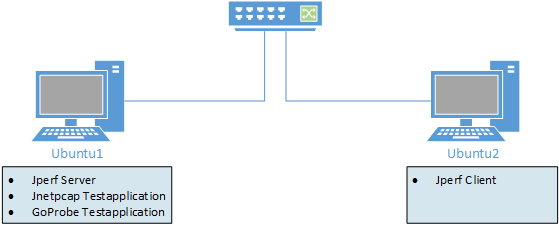
\includegraphics[width=0.7\textwidth]{start/img/PerformanceEvaluation.png}

Der Datenverkehr wurde mithilfe von Jperf simuliert und jeweil mit den beiden Testapplikationen aufgezeichnet.\\
Für Java wurde eine Testapplikation mit der Library JnetPcap erstellt. JnetPcap ist eine Opensource Library die einen wrapper für die Libpcap-Library zur verfügung stellt.\\
Für Go wurden die Pakete mithilfe von GoProbe aufgezeichnet. GoProbe ist ebenfalls Opensource und verwendet die Libpcap-Library.

\subsection{Performancetest Resultat}
Auslastung des Prozessors...

=======
\section{Einführung}
Gemäss der Aufgabenstellung dieser \work ist die Programmiersprache für das \tool frei wählbar mit der einzigen Voraussetzung dass man eine \acs{PCAP}-Library einbinden kann. In der Inception-Phase des Projekts ging es daher darum eine geeignete Sprache und Bibliothek zu wählen.

\section{JNetPcap}
\label{sec:JNetPcap}

todo Jan

\section{Golang und goPacket}
\label{sec:Golang und goPacket}

\subsection{Golang}
Golang, auch Go genannt, ist eine eher junge Programmiersprache seit 2007 von Google Inc. entwickelt wurde. Golang hat einen C-ähnlichen Syntax, bietet aber viele Eigenschaften von modernen Programmiersprachen wie zum Beispiel Garbage Collection, Type-Safety, Dynamic-Typing, Closures und eine grosse Standard-Library.
Im Oktober 2009 wurde die Golang der Öffentlichkeit als Open Source zur Verfügung gestellt.

\subsection{Evaluation}
Unseren ersten Kontakt mit Golang haben wir durch GoProbe von Open Systems gewonnen.
GoProbe erlaubt leichtgewichtiges aggregieren von Paketen und deren effiziente Speicherung. Eine Abfrage der gespeicherten Paketen ist via Querying Flows möglich.


\section{Performance Vergleich}
\label{sec:Performance Vergleich}

\subsection{Testaufbau}
2 Desktop-Rechner der HSR sind via Gigabit-Lan miteinander verbunden. Auf den Rechnern läuft Ubuntu 14.04 x64 sowie jPerf und die jeweils getestete Software.

%todo Grafik mit MS Visio die unser Testaufbau darstellt.

\subsection{Testdurchführung}
Auf einem der beiden Rechnern läuft jeweils jPerf im Server-Modus sowie die getestete Software. Auf dem anderen Computer läuft jPerf im Client-Modus.
Via. jPerf wird nun soviel Traffic erzeugt um die 1Gbit/s-Leitung möglichst stark auszulasten, d.h. durchschnittlich 900mbit/s. Die getestete Software zeichnet dabei die ganzen Pakete auf und sollte dabei 300mbit/s an Traffic ertragen können. 300mbit/s sind gem. Open Systems AG die Lastspitzen mit denen etwa zu rechnen sind.

\subsection{Ergebnisse}
Java und Golang sind von den Ergebnissen her recht ähnlich. Beide haben die Anforderung von 300mbit/s erfolgreich erfüllt. Golang ist mit den Durchschnittlich 17\% CPU Auslastung etwas performanter als Java. Die 31\% CPU Lastspitze bei Java gibt es jeweils nur wenn das Programm zum ersten Mal gestartet wird und kommt daher dass dann die ganze \acs{JVM} zuerst hochgefahren werden muss.
Beim Memory siehts bei goProbe klar besser aus weil es den ganzen \acs{JVM} Overhead nicht hat.

\begin{table}[h]
\begin{tabular}{|l|l|l|l|}
\hline
\rowcolor[HTML]{C0C0C0} 
\textbf{Software} & \textbf{CPU Spitze} & \textbf{CPU Ø} & \textbf{Memory Ø} \\ \hline
JNetPcap auf Java & 31\%                & 20\%           & tbd               \\ \hline
goProbe auf Go    & 18\%                & 17\%           & tbd               \\ \hline
\end{tabular}
\end{table}

\section{Entscheidung}
Open Systems AG würde es bevorzugen wenn wir Golang statt Java einsetzen. Die Ergebnisse des Performance-Tests sprechen ebenfalls für Golang. Und wir haben durchaus auch das Interesse einmal eine neue Programmiersprache zu lernen.
In Anbetracht dessen haben wir uns entschieden das \tool mit Golang zu entwickeln.
>>>>>>> origin/master
